\section{Unknown mixtures and passive data}\label{sec:mixtures}

Theorem~\ref{thm:quantity} concerns a \emph{known} pair. A supervisor faces an unknown number of cohorts with unknown rates and weights. This section asks how fast the cost of recovering them grows.

\subsection{Why naive pole fitting fails}

Because the memory rates are zeros of $H$ (Theorem~\ref{thm:merged}), extracting poles directly from the price impulse response by matrix-pencil or Prony methods targets closed-loop eigenvalues. A four-step inversion repairs this: (1) decouple $g_t=h_{t+1}-ah_t$; (2) form a Hankel matrix of $g$ and compute a minimal realization by Kung's eigensystem realization; (3) compute its transmission zeros, which are the roots of the denominator of $G$; (4) project reconstructed flow onto the recovered memory filters to obtain the weights (Appendix~\ref{app:era}). Without noise this recovers $K=0$, $K=1$ and well-separated two-cohort systems exactly (Appendix~\ref{app:era}); with noise, per-cohort weights become unreliable once rates are close. The reason is information-theoretic, as the rest of this section shows.

\subsection{Local information: the Cram\'er--Rao benchmark}

\begin{proposition}[Cram\'er--Rao benchmark]\label{prop:crb}
Let $\theta$ collect the weights $w_1,\ldots,w_K$ and rates $\eta_1,\ldots,\eta_K$. Suppose the impulse response $h_t(\theta)$, $t\le T$, is observed with i.i.d.\ Gaussian error from $N$ reset probes of size $V_{\rm probe}$ against innovation noise $\sigma_p$, so the error has standard deviation $\sigma_h=\sigma_p/(V_{\rm probe}\sqrt N)$. With Jacobian $J_{tj}=\partial h_t/\partial\theta_j$ and $F_{\rm unit}=J^\top J$, any regular unbiased estimator has ${\rm Var}(\hat w_k)\ge\sigma_h^2[F_{\rm unit}^{-1}]_{kk}$, and a 95\% interval of half-width ${\rm tol}$ requires
\begin{equation}\label{eq:Ncrb}
N^*\ge\Bigl(\frac{1.96}{\rm tol}\Bigr)^2\Bigl(\frac{\sigma_p}{V_{\rm probe}}\Bigr)^2[F_{\rm unit}^{-1}]_{kk}.
\end{equation}
For $K=2$ with spacing $\Delta\eta$, $[F_{\rm unit}^{-1}]_{kk}=\Theta((\Delta\eta)^{-6})$, so $N^*=\Theta((\Delta\eta)^{-6})$.
\end{proposition}

\paragraph{In words.} This gives the number of test trades any well-behaved estimator needs to pin down one group's trading weight to a stated precision. Each extra group with a nearby memory raises the number sharply, as Table~\ref{tab:crb} shows.

\begin{table}[t]\centering\small
\begin{threeparttable}
\caption{Cram\'er--Rao sample sizes for multi-cohort weight recovery ($T=120$ taps)}\label{tab:crb}
\begin{tabular}{lcrccc}
\toprule
Scenario & $K$ & $N^*$ probes & $\sigma_{\rm crit}$ & ML success ($f=1$) & RMSE/CRB\\
\midrule
$\eta=0.30$ & 1 & 0.1 & $6.05\times10^{-3}$ & 94\% & 1.02\\
$\Delta\eta=0.30$ & 2 & 47.8 & $2.31\times10^{-4}$ & 94\% & 1.01\\
$\Delta\eta=0.20$ & 2 & 597 & $6.55\times10^{-5}$ & 96\% & 0.98\\
$\Delta\eta=0.10$ ($\delta=0.05$ pair) & 2 & 40{,}374 & $7.96\times10^{-6}$ & 93\% & 1.03\\
$\Delta\eta=0.05$ & 2 & 2{,}620{,}320 & $9.88\times10^{-7}$ & 95\% & 1.03\\
spacing 0.10 & 3 & 17{,}349{,}791 & $3.84\times10^{-7}$ & 98\% & 1.22\\
spacing 0.20 & 3 & 27{,}038 & $9.73\times10^{-6}$ & 98\% & 0.88\\
\bottomrule
\end{tabular}
\begin{tablenotes}\footnotesize\item Tolerance $\pm0.01$ at 95\%. $\sigma_{\rm crit}$ is the single-probe noise at which one probe suffices; operational single-probe noise is $1.6\times10^{-3}$. ML columns: least squares over all weights and rates from six generic starts (never the true values), 200 replications per row at $\sigma_{\rm crit}$; success means every weight within $\pm0.01$. Fitted log--log slope of $N^*$ in $\Delta\eta$: $-6.04$. \end{tablenotes}
\end{threeparttable}
\end{table}

At the critical noise level maximum likelihood attains the bound: its RMSE for the hardest weight is between 0.88 and 1.22 times the Cram\'er--Rao value and every weight is within tolerance in 93\% to 98\% of replications (Table~\ref{tab:crb}), so the critical noise levels, not estimator failure, are what make close cohorts expensive. Under ordinary surveillance budgets ($N\le50$) unbiased estimators cannot resolve close weights.

\subsection{A global two-point bound for any estimator}

The Cram\'er--Rao benchmark of Proposition~\ref{prop:crb} applies only to regular unbiased estimators. Could biased, ridge, shrinkage or Bayesian estimators escape the $(\Delta\eta)^{-6}$ scaling? No.

\begin{theorem}[Global two-point bound and matching upper bound, $K=2$]\label{thm:twocohort}
In this theorem $w_k$ denotes cohort $k$'s trading intensity $q_k$, not the merged weight $q_k\eta_k$ of Section~\ref{sec:model}, and $\Delta\eta$ is the actual spacing of the two rates. Fix total intensity $q=0.20$, mean rate $\bar\eta=0.40$, target separation $\tau=0.01$, and $\Delta\eta\in(0,8/11)$ (so that $\bar\eta-p_+\Delta\eta>0$). Let $p_\mp=\tfrac12\mp\tau/q$ and
\begin{equation}\label{eq:pair}
\theta_0=(qp_-,qp_+,\bar\eta-p_+\Delta\eta,\bar\eta+p_-\Delta\eta),\qquad\theta_1=(qp_+,qp_-,\bar\eta-p_-\Delta\eta,\bar\eta+p_+\Delta\eta).
\end{equation}
\begin{enumerate}[label=(\roman*)]
\item Label cohorts in increasing order of rate, so that weight vectors are compared rate by rate (as unordered sets the two weight vectors coincide). Both economies have spacing $\Delta\eta$, weight separation $\|w(\theta_1)-w(\theta_0)\|_\infty=2\tau$ in this labelling, and equal rate moments $M_m=\sum_kw_k\eta_k^m$ for $m\in\{0,1,2\}$, while
\begin{equation}\label{eq:dM3}
M_3(\theta_1)-M_3(\theta_0)=4\tau p_-p_+(\Delta\eta)^3 .
\end{equation}
Hence $\|h(\theta_1)-h(\theta_0)\|_2=\Theta(\tau(\Delta\eta)^3)$.
\item For any measurable estimator (including biased, ridge, James--Stein or MAP) that reports weights in the same rate order, the supremum being over the class of two-cohort economies with total weight $q$, mean rate $\bar\eta$ and spacing $\Delta\eta$,
\begin{equation}\label{eq:lecam2}
\sup_\theta P_\theta(\|\hat w-w(\theta)\|_\infty\ge\tau)\;\ge\;1-\Phi\!\Bigl(\frac{\sqrt N\|h(\theta_1)-h(\theta_0)\|_2}{2\sigma_h}\Bigr),
\end{equation}
so failure probability at most $0.05$ requires $N\ge4\sigma_h^2z_{0.95}^2/\|h(\theta_1)-h(\theta_0)\|_2^2=\Omega((\Delta\eta)^{-6})$. For $\Delta\eta\ge2\tau q/(q+2\tau)$ ($\approx0.018$ at the stated values) the same bound holds without any labelling convention, for the permutation-invariant loss
\[
d_\infty(\hat\theta,\theta)=\min_{\pi\in S_2}\max_{k}\bigl(|\hat w_{\pi(k)}-w_k|+|\hat\eta_{\pi(k)}-\eta_k|\bigr),
\]
because then $d_\infty(\theta_0,\theta_1)=\min\{2\tau(1+\Delta\eta/q),\,(1+2\tau/q)\Delta\eta\}\ge2\tau$. For smaller spacings the relevant permutation-invariant statement is the Wasserstein bound of Theorem~\ref{thm:kcohort}.
\item Conversely, the matching upper bound $N=O((\Delta\eta)^{-6})$ on rich separated two-cohort classes is Theorem~\ref{prop:esprit} with $K=2$. On the separated class with weights and rates bounded away from the boundary, Toeplitz deconvolution followed by a Prony--Hankel root step has Hankel determinant $g_1g_3-g_2^2=w_1w_2\eta_1\eta_2r_1r_2(\Delta\eta)^2>0$ for the deconvolved kernel $g_m=\sum_iw_i\eta_ir_i^m$, and perturbation analysis gives the same order.
\end{enumerate}
\end{theorem}

\paragraph{In words.} For two unknown groups, no method can tell the two candidate markets apart reliably with fewer than a number of experiments of order $(\Delta\eta)^{-6}$, and a practical method (Prony's method, Theorem~\ref{prop:esprit}) achieves this order. Halving the spacing multiplies the data needed by 64.

We recomputed the two-point quantities exactly (Table~\ref{tab:lecam}): the moment gap equals $4\tau p_-p_+(\Delta\eta)^3$ to machine precision, and the Le Cam requirement at $\Delta\eta=0.10$ is $5{,}927.6$ resets. The worst-case failure rates of four re-implemented estimators all lie above the lower bound (Table~\ref{tab:lecam}).

\begin{table}[t]\centering\small
\begin{threeparttable}
\caption{Two-point sample complexity for two-cohort weight recovery}\label{tab:lecam}
\begin{tabular}{lcccc}
\toprule
$\Delta\eta$ & $\Delta M_3$ & $\|\Delta h\|_2$ & $N^*_{\rm LeCam}$ (95\%) & $N^*_{\rm CRB}$\\
\midrule
0.30 & $2.67\times10^{-4}$ & $1.98\times10^{-3}$ & 7.1 & 47.8\\
0.20 & $7.92\times10^{-5}$ & $5.60\times10^{-4}$ & 88.2 & 597.0\\
0.14 & $2.72\times10^{-5}$ & $1.89\times10^{-4}$ & 775.3 & 5{,}267.9\\
0.10 & $9.90\times10^{-6}$ & $6.84\times10^{-5}$ & 5{,}927.6 & 40{,}374.2\\
0.08 & $5.07\times10^{-6}$ & $3.49\times10^{-5}$ & 22{,}740.5 & 155{,}048.9\\
0.06 & $2.14\times10^{-6}$ & $1.47\times10^{-5}$ & 128{,}333.0 & 875{,}732.3\\
0.05 & $1.24\times10^{-6}$ & $8.50\times10^{-6}$ & 383{,}859.1 & 2{,}620{,}321.2\\
0.04 & $6.34\times10^{-7}$ & $4.35\times10^{-6}$ & 1{,}466{,}361.5 & 10{,}012{,}662.4\\
\midrule
\multicolumn{5}{p{0.85\textwidth}}{\emph{Worst-case failure at $\Delta\eta=0.10$, $N=50$, 1,000 trials per hypothesis}: bound 44.1\%; ML 94.5\%, ridge 47.5\%, positive-part shrinkage 100\%, heavy prior 73.9\%.}\\
\bottomrule
\end{tabular}
\begin{tablenotes}\footnotesize\item $\tau=0.01$, $\sigma_h=1.6\times10^{-3}$, $a=0.5$, $\kappa=0.8$, 121 taps. Recomputed columns from \texttt{recompute\_theory.py}. Estimators re-implemented in \texttt{recompute\_p1\_estimators.py}: ML is least squares from four starts; ridge and heavy prior are posterior modes with prior standard deviations $(0.05,0.10)$ and $(0.005,0.02)$ for (weights, rates) around the symmetric centre of the two hypotheses; positive-part shrinkage pulls the ML weights toward their mean. Failure means some weight is off by at least $\tau$.\end{tablenotes}
\end{threeparttable}
\end{table}

\begin{remark}[The hard directions carry no risk]\label{rem:riskneutral}
The two economies of Theorem~\ref{thm:twocohort} have the same total weight $\sum_iq_i=q$, so their summed price response $\sum_th_t=\kappa/(1-a-\kappa\sum_iq_i)$ is identical, $2.353$ at the calibration of Table~\ref{tab:lecam}: the directions in which prices are least informative about the cohorts are directions in which cumulative price risk does not move. The summed response is a linear functional of the response and is estimated at the parametric rate whatever the spacing of the memories; the companion paper turns this into a certification theorem, a minimax-optimal pre-trade guard and a decision value of disclosure \citep{niroula2026b}. Identification and safety ask different questions of the same data.
\end{remark}

\subsection{Many unknown cohorts}

\begin{theorem}[$K$-cohort two-point lower bound]\label{thm:kcohort}
Fix $K\ge2$, a center $r_c\in(0,1)$, total merged weight $W>0$ and $0<\Delta\eta<\min(r_c,1-r_c)$, so that all rates lie in $(0,1)$, and assume $a+\kappa W/(1-r_c-\Delta\eta)<1$, so that every candidate economy is Schur stable. Each reset experiment observes $T\ge2K$ noisy taps ($T=\infty$ allowed); the bound below uses the full response norm, which dominates any finite prefix. There exist two $K$-cohort economies with rates in $r_c+\Delta\eta[-1,1]$, positive weights, and merged measures whose moments of order $0,\ldots,2K-2$ coincide while the moment of order $2K-1$ differs by a constant times $(\Delta\eta)^{2K-1}$. Their impulse responses differ by $\|h^A-h^B\|_2\asymp(\Delta\eta)^{2K-1}$, so recovering the weights from $N$ independent noisy reset experiments with worst-case error probability below $1/4$ requires
\[
N\;\ge\;c\,\sigma^2(\Delta\eta)^{-(4K-2)} .
\]
The same requirement holds for the permutation-invariant loss $W_1(\hat M,M)$ between estimated and true merged measures at accuracy $c_KW\Delta\eta$, where $2c_K>0$ is the Wasserstein distance between the two normalized quadrature rules, so no relabelling of atoms escapes it.
\end{theorem}

The two losses have different targets. The weights of the two economies differ by a constant that does not shrink with $\Delta\eta$, so the first statement is about weights at fixed accuracy, which Theorem~\ref{prop:esprit} matches; the Wasserstein statement is about the memory distribution at accuracy proportional to $\Delta\eta$, which Theorem~\ref{thm:uniformw1} matches.

The construction uses the $K$-point Gauss and Gauss--Radau rules of the same weight function: both are positive, have $K$ atoms and integrate polynomials of degree $2K-2$ exactly. For $K=2$ it reproduces the order of Theorem~\ref{thm:twocohort}. Table~\ref{tab:radau} lists the two rules: their low moments agree to machine precision and their moment of order $2K-1$ differs by $0.222$, $0.0533$ and $0.0131$ for $K=2,3,4$. The shrinking gap explains why constants deteriorate with $K$ on top of the exponent.

\paragraph{What counts as an experiment.} In Theorem~\ref{thm:kcohort} an experiment is a unit impulse from the reset state whose response is observed with noise of variance $\sigma^2$ per tap. The exponent is the same for any probe design of bounded energy. For any probe $v$ the mean difference between the two economies is at most $\sup_\omega|\Delta\hat H(e^{i\omega})|\,\|v\|_2$, and $\sup_\omega|\Delta\hat H|=O((\Delta\eta)^{2K-1})$ because $\Delta\hat H=z^{-1}\hat H_A\hat H_B\,\Delta G$ with both responses bounded on the circle. Experiments with probe energy $E$ each therefore need $NE\gtrsim\sigma^2(\Delta\eta)^{-(4K-2)}$: a larger probe buys the same information with fewer experiments, and Section~\ref{sec:account} prices the capital that a larger probe requires. The bound does not cover information obtained without trading against the groups, such as class records (Section~\ref{sec:disclosure}).

\begin{table}[t]\centering\small
\begin{threeparttable}
\caption{Gauss and Gauss--Radau rules on $[-1,1]$ used in Theorem~\ref{thm:kcohort}}\label{tab:radau}
\begin{tabular}{cp{0.42\textwidth}cc}
\toprule
$K$ & Gauss nodes / Gauss--Radau nodes & Max gap, orders $<2K-1$ & Gap at order $2K-1$\\
\midrule
2 & $\pm0.5774$ \;/\; $-1,\ 0.3333$ & $6\times10^{-17}$ & 0.2222\\
3 & $0,\ \pm0.7746$ \;/\; $-1,\ -0.2899,\ 0.6899$ & $2\times10^{-16}$ & 0.0533\\
4 & $\pm0.3400,\ \pm0.8611$ \;/\; $-1,\ -0.5753,\ 0.1811,\ 0.8228$ & $4\times10^{-16}$ & 0.0131\\
\bottomrule
\end{tabular}
\begin{tablenotes}\footnotesize\item All Gauss--Radau weights are positive. \end{tablenotes}
\end{threeparttable}
\end{table} Table~\ref{tab:kcohort} and Figure~\ref{fig:kcohort} confirm the order numerically.

\begin{table}[t]\centering
\begin{threeparttable}
\caption{Numerical check of Theorem~\ref{thm:kcohort}}\label{tab:kcohort}
\begin{tabular}{lccc}
\toprule
 & $K=2$ & $K=3$ & $K=4$\\
\midrule
Theoretical exponent of $N^*$ & $-6$ & $-10$ & $-14$\\
Fitted log--log slope (small $\Delta\eta$) & $-5.96$ & $-9.96$ & $-14.01$\\
\bottomrule
\end{tabular}
\begin{tablenotes}\footnotesize
\item Le Cam bound $N^*\propto\sigma^2/\|h^A-h^B\|_2^2$ with $\sigma=1$, $a=0.5$, $\kappa=1$, total merged weight $0.10$, rates centered at $0.70$, responses over 400 lags. \end{tablenotes}
\end{threeparttable}
\end{table}

\begin{figure}[t]\centering
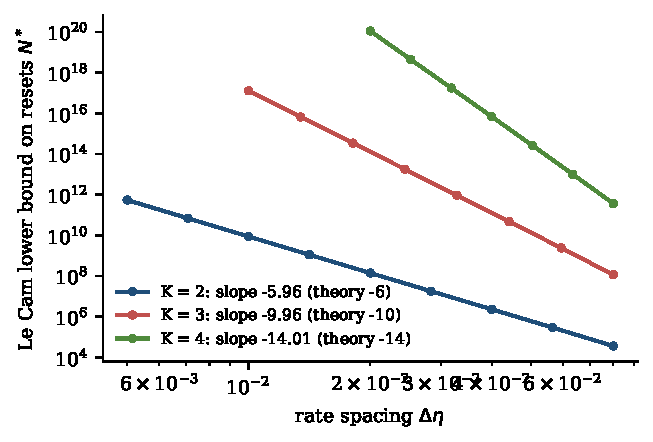
\includegraphics[width=0.62\textwidth]{figs/fig_kcohort.pdf}
\caption{Two-point lower bound on the number of reset experiments needed to separate $K$-cohort economies, as a function of the rate spacing.}\label{fig:kcohort}
\end{figure}

\begin{theorem}[Matching upper bound for every $K$]\label{prop:esprit}
Fix $K\ge2$, a compact set $\mathcal S\subset\{s\in[-1,1]^K:s_1<\cdots<s_K\}$ of ordered rescaled rates with $\min_{i\ne j}|s_i-s_j|\ge\gamma>0$, and merged weights $w_i\in[\omega_{\min},\omega_{\max}]$ with $\omega_{\min}>0$. Consider the class of $K$-cohort economies with rates $r_c+\Delta\eta\,s$, $s\in\mathcal S$, and $N$ independent reset experiments whose responses carry Gaussian noise with variance $\sigma^2$. There are constants $c_0,C>0$ depending only on $(K,\mathcal S,\gamma,\omega_{\min},\omega_{\max},a,\kappa,r_c)$ such that, whenever $\epsilon_N\equiv\sigma N^{-1/2}(\Delta\eta)^{-(2K-1)}\le c_0/\sqrt{\log(4K/\beta)}$, Prony's method applied to the first $2K$ estimated kernel values, with its output atoms listed in increasing order of rate, recovers the weights with
\[
\max_i|\hat w_i-w_i|\;\le\;C\sqrt{\log(4K/\beta)}\;\epsilon_N
\]
with probability at least $1-\beta$. Hence $N=C'\sigma^2(\Delta\eta)^{-(4K-2)}$ experiments suffice for any fixed accuracy and confidence. On any such class that contains the Gauss and Gauss--Radau pair of Theorem~\ref{thm:kcohort} (a rich class), together with that theorem the minimax sample requirement is $N^*\asymp\sigma^2(\Delta\eta)^{-(4K-2)}$. On smaller classes the upper bound need not be tight: if the rates are known, for example, the weights need only order $\sigma^2(\Delta\eta)^{-2}$ experiments. The constants $c_0$ and $C$ grow quickly with $K$, through the conditioning of the moment map; the theorem gives the order in $\Delta\eta$ for fixed $K$, not a usable constant for large $K$ (in Supplement Table~\ref{tab:stress} our double-precision Prony implementation already fails at $K=4$ on the disclosure grid).
\end{theorem}

\begin{proof}
The kernel values $k_m=\sum_iw_ir_i^m$ are the power moments of the merged measure. The closed-loop recursion $h_t=ah_{t-1}+\kappa\sum_mk_mh_{t-1-m}$ (plus $\kappa$ at $t=0$) can be solved for $k_0,\ldots,k_{2K-1}$ from $h_1,\ldots,h_{2K}$. Because $h_0=\kappa$ is a known primitive, each $k_m$ is a polynomial in $h_1,\ldots,h_{m+1}$ with coefficients depending on $(a,\kappa)$ (the only division is by $\kappa h_0=\kappa^2$), so on the bounded set of responses within sup-distance $1$ of the class this map is $L_h$-Lipschitz, with $L_h$ depending on the class but not on $\Delta\eta$. Let $E$ be the event $\max_{1\le t\le2K}|\bar h_t-h_t|\le\sigma N^{-1/2}\sqrt{2\log(4K/\beta)}$, where $\bar h_t$ averages the $N$ responses; a Gaussian tail bound and a union bound over the $2K$ estimated taps give $P(E)\ge1-\beta$. On $E$, and provided this radius is at most $1$, the estimated kernel values satisfy $\max_m|\hat k_m-k_m|\le L_h\sigma N^{-1/2}\sqrt{2\log(4K/\beta)}$. Centring at $r_c$ is a fixed triangular linear map, $\mu_m=\sum_{j\le m}\binom mj(-r_c)^{m-j}k_j$, and $\mu_m=(\Delta\eta)^m t_m$ with $t_m=\sum_iw_is_i^m$. The map $F:(s,\omega)\mapsto(t_0,\ldots,t_{2K-1})$ does not depend on $\Delta\eta$; its Jacobian is a confluent Vandermonde matrix with determinant $\prod_i\omega_i\prod_{i<j}(s_i-s_j)^4$, bounded away from zero on the compact class. On ordered, $\gamma$-separated nodes $F$ is injective, because a measure with $K$ distinct atoms is determined by its first $2K$ moments. A $C^1$ map that is injective on a compact set $Q$ and has a nonsingular Jacobian there is injective on an open neighbourhood $U$ of $Q$: otherwise there are $x_n\ne y_n$ with $F(x_n)=F(y_n)$ and distance to $Q$ tending to zero, whose limits $x,y\in Q$ satisfy $F(x)=F(y)$, so $x=y$, contradicting local injectivity at $x$. Applying the quantitative inverse function theorem uniformly on $Q$, there are $\rho_0>0$ and $L<\infty$, uniform over the class, such that $F(U)$ contains the ball of radius $\rho_0$ around every point of $F(Q)$ and the single inverse $F^{-1}:F(U)\to U$ is $L$-Lipschitz on each such ball. An error $e$ in $\mu_m$ is an error $e(\Delta\eta)^{-m}$ in $t_m$, largest at $m=2K-1$. Since $\Delta\eta<1$ and the centring map is fixed, on $E$ we get $\|\hat t-t\|_\infty\le C_1\sqrt{\log(4K/\beta)}\,\epsilon_N$ with $C_1$ equal to $\sqrt2L_h$ times the norm of the centring map; and because $\sigma N^{-1/2}\sqrt{2\log(4K/\beta)}\le\sqrt2\,\epsilon_N\sqrt{\log(4K/\beta)}$, the radius condition holds whenever $c_0\le1/\sqrt2$. When this is below $\rho_0$, $\hat t$ lies in the ball where $F^{-1}$ is $L$-Lipschitz. For an input in such a ball, $x=F^{-1}(\hat t)$ has $K$ distinct nodes and nonzero weights, so the $K\times K$ Hankel matrix of $\hat t$ is nonsingular and Prony's method returns exactly $x$: the Prony polynomial is determined uniquely by the Hankel system, and since the $K$ real nodes of $x$ reproduce $\hat t$ it equals $\prod_i(z-\hat s_i)$, so its roots are real and distinct and no complex pair can appear; Prony's method computes the algebraic inverse of the moment map up to the order of the atoms, so, listing its output in increasing order of rate (which the error bound below keeps unambiguous once $C\sqrt{\log(4K/\beta)}\,\epsilon_N<\gamma/2$), its output is $F^{-1}(\hat t)$ and the stated bound follows with $C=LC_1$ and $c_0=\min\{\min(\rho_0,\gamma/(2L))/C_1,\,1/\sqrt2\}$, which also keeps $C\sqrt{\log(4K/\beta)}\,\epsilon_N<\gamma/2$. No separate root-perturbation bound is needed: on the ball where $F^{-1}$ is $L$-Lipschitz, Prony's roots and weights are the coordinates of $F^{-1}(\hat t)$, so the conditioning of the root step is part of $L$ (for an explicit step-by-step analysis of Prony's method with clustered exponents see \citealp{katz2023}). The matching statement requires the class to contain the Gauss and Gauss--Radau pair of Theorem~\ref{thm:kcohort} (ordered nodes with separation at least the smaller of their two minimum gaps, and weights within $[\omega_{\min},\omega_{\max}]$ after scaling to total weight $W$); for any such class the orders match, with constants that depend on the class.
\end{proof}

\paragraph{In words.} With $K$ unknown groups whose memories lie within $\Delta\eta$ of each other, the number of experiments needed grows like $(\Delta\eta)^{-(4K-2)}$. For two groups, halving the spread multiplies the data needed by 64; for three groups, by 1{,}024. Theorem~\ref{thm:kcohort} shows that no method does better, and this theorem shows that Prony's method achieves it.

\paragraph{Machine check.} Lean verifies this theorem for every $K\ge1$ (\texttt{p1\_thm\_prony\_upper\_bound}), using only Lean's standard axioms. The formal proof follows the one above: a Lipschitz bound for the closed-loop deconvolution that does not depend on $\Delta\eta$, the $(\Delta\eta)^{-m}$ rescaling, a sub-Gaussian tail bound over the $2K$ taps, injectivity of the Jacobian of the moment map (proved by Hermite interpolation, without the determinant formula), and a uniform inverse function theorem on the compact class. The formal estimator is the representation with increasing nodes and nonzero weights that matches the $2K$ estimated moments; Lean shows that it is unique and that Prony's linear system has a unique solution whose polynomial has exactly its nodes as roots, so the roots are real. The formal statement allows sub-Gaussian noise and assumes $|r_c|+\Delta\eta\le1$, so that every memory rate has modulus at most one.


Table~\ref{tab:kupper} confirms the order numerically. For numerical stability the estimator works in centred and rescaled coordinates (the estimator is the same; only its floating-point evaluation changes). The argument parallels the stability analysis of super-resolution for clustered complex nodes \citep{batenkov2021}, and \citet{katz2023} show that Prony's method attains the min-max bound for clustered exponents; here the nodes are real and are first extracted from the closed loop, and it reproduces the ESPRIT slope of $-6.15$ reported for $K=2$ in the earlier version.

\begin{table}[t]\centering\small
\begin{threeparttable}
\caption{Sample requirement of Prony's method against the lower-bound order}\label{tab:kupper}
\begin{tabular}{lcccc}
\toprule
 & $K=2$ & $K=3$ & $K=4$ & $K=5$\\
\midrule
Lower-bound order $-(4K-2)$ & $-6$ & $-10$ & $-14$ & $-18$\\
Fitted slope of $N^*$ in $\Delta\eta$ (Prony) & $-5.94$ & $-10.00$ & $-13.93$ & $-18.34$\\
\bottomrule
\end{tabular}
\begin{tablenotes}\footnotesize\item Rates $0.7+\Delta\eta\,s$ with $s$ the $K$-point Gauss nodes, total weight 0.1, $\Delta\eta\in[0.03,0.2]$; $N^*$ is the number of experiments for a weight RMSE of 10\% of the smallest weight, from 400 simulated estimates per point. At $K=5$ the fit is numerically sensitive: rerunning the same seeded script with a different numerical library gives slopes $-5.94$, $-10.00$, $-13.92$ and $-17.89$. \end{tablenotes}
\end{threeparttable}
\end{table}

\subsection{Do the rates survive real market noise?}\label{sec:injection}

Theorems~\ref{thm:kcohort} and~\ref{prop:esprit} are proved for observation errors that are independent and Gaussian, and Table~\ref{tab:kupper} checks them with Gaussian noise. Real price changes are different: one-minute returns have heavy tails, although they are almost uncorrelated from one minute to the next. To see whether the rates depend on the Gaussian assumption, we ran a pre-specified test (SHA-256 \texttt{596a700da2e4\ldots}, opened once) in which the trader groups are synthetic, with known memory spacing, and only the noise is real. Each reset experiment returns the price response to a unit impulse plus a window of consecutive one-minute log-price changes of Binance BTCUSDT, demeaned and scaled to unit variance. The changes come from 21 days, the 6th of each month from January 2025 to September 2026, that are used nowhere else in this project; their kurtosis is 19.4, against 3 for Gaussian noise. With class tagging, the experiment also returns each group's flow response, observed through independent windows of the same noise. A control arm uses i.i.d.\ Gaussian noise of the same variance. For each spacing, $N^*$ is the smallest number of experiments at which every recovered weight lies within 25\% of the smallest true weight in at least 75\% of 200 replications, using Prony's method on prices alone or the per-group regression of Proposition~\ref{prop:tagged} with tagging. The noise level and the spacing grids were fixed on Gaussian noise alone, before any real noise was downloaded.

\begin{table}[t]\centering\small
\begin{threeparttable}
\caption{Sample requirement with real Bitcoin price noise: fitted slope of $\log N^*$ in $\log\Delta\eta$}\label{tab:injection}
\begin{tabular}{lccccl}
\toprule
 & Theory & Real noise & Gaussian control & Pre-specified criterion & Result\\
\midrule
Price only, $K=2$ (H1) & $-6$ & $-6.01$ & $-6.22$ & slope in $[-7.5,-4.5]$ & pass\\
Tagged, $K=2$ (H2) & bounded & 256--724 & 256--1{,}024 & max/min $\le8$ & pass (2.8)\\
Price only, $K=3$ (H3) & $-10$ & $-9.81$ & $-9.96$ & slope in $[-12.5,-7.5]$ & holds\\
\bottomrule
\end{tabular}
\begin{tablenotes}\footnotesize\item Synthetic groups at rates $r_c+\Delta\eta\,s$ ($s$ the $K$-point Gauss nodes; $r_c=0.6$ and $\Delta\eta$ from 0.5 to 0.125 for $K=2$, $r_c=0.5$ and $\Delta\eta$ from 0.6 to 0.25 for $K=3$), $a=0.5$, $\kappa=0.8$, total weight 0.08, $\sigma=10^{-3}$, $\sigma_f=0.02$. The test passes if H1 and H2 hold; H3 is reported either way. The tagged row gives the range of $N^*$ over the spacing grid. Requirements above $4{,}096$ use the central-limit draw described in the text. Requirements at each spacing are in Supplement Table~\ref{tab:injectionfull}. Specification SHA-256 \texttt{596a700da2e4\ldots}; opened once. Kind: semi-synthetic (synthetic groups, real noise).\end{tablenotes}
\end{threeparttable}
\end{table}

Both pre-specified hypotheses hold, so the test passes (Table~\ref{tab:injection}). With real noise, the price-only requirement for two groups rises from 64 experiments at $\Delta\eta=0.5$ to $370{,}728$ at $\Delta\eta=0.125$, a factor of about 5{,}800, and the fitted slope is $-6.01$; for three groups it is $-9.81$. Over the same grid the tagged requirement stays between 256 and 724 experiments, and it falls slightly rather than rises as the spacing shrinks. At every spacing the real-noise requirement is within one step of the grid (a factor $\sqrt2$) of the Gaussian control.

The test has a limit, stated in its specification. Averages of $N$ real windows are resampled exactly up to $N=4{,}096$; beyond that they are drawn as Gaussian vectors with the real windows' covariance, as the central limit theorem suggests. Real one-minute changes are almost uncorrelated (lag-one autocorrelation between $-0.007$ and $0.009$ within the windows), so beyond $4{,}096$ the real and Gaussian arms differ little by construction. The direct evidence about heavy tails therefore comes from the points in the exact range: every tagged requirement, and the price-only requirements for two groups at the three widest spacings (64, 362 and 1{,}448 experiments, against 64, 362 and 1{,}024 with Gaussian noise). The other four price-only points for two groups, and all points for three groups, check the rate with the real noise's variance and covariance but not its tails. Averaging should make heavy tails matter less as $N$ grows, but the test does not show this.

\paragraph{In words.} Where real Bitcoin price noise could be used directly, it needs about as many experiments as Gaussian noise, and over the whole grid halving the spacing between two groups still multiplies the number of experiments by about 64, while class-tagged records keep the requirement flat. At the largest sample sizes the test relies on a normal approximation to the real noise.

\subsection{Near-colliding rates: a uniform rate for the merged measure}\label{sec:uniform}

Theorem~\ref{prop:esprit} needs the rates to stay $\gamma$-separated and every weight to stay away from zero. Neither restriction can be dropped for weight recovery: two atoms of weights $w$ and $W-w$ at rates $r$ and $r+\Delta$ and two of weights $W-w$ and $w$ at the same rates have merged measures that converge to the same measure as $\Delta\to0$, so no estimator recovers the individual weights uniformly over near-colliding economies. What can be recovered uniformly is the merged measure itself, in the permutation-invariant Wasserstein distance.

\begin{theorem}[Uniform rate without separation]\label{thm:uniformw1}
Fix $K\ge1$, a memory bound $\bar r<1$ and $0<m_{\min}\le B$. Let $\mathcal M_K$ be the merged measures with at most $K$ atoms in $[0,\bar r]$ and total mass $k_0\in[m_{\min},B]$, with no separation condition and no lower bound on individual weights, and write $\bar M=M/k_0$ for the normalized memory distribution. From $N$ reset experiments as in Theorem~\ref{prop:esprit}, let $\hat M$ be any element of $\mathcal M_K$ whose first $2K$ kernel values are closest in the sup norm to the estimated ones. There is $C$ depending only on $(K,\bar r,a,\kappa,B)$ such that, with probability at least $1-\beta$,
\[
W_1(\hat{\bar M},\bar M)\;\le\;C\Bigl(\frac{\sigma\sqrt{\log(4K/\beta)}}{m_{\min}\sqrt N}\Bigr)^{1/(2K-1)}\qquad\text{uniformly over }\mathcal M_K .
\]
Hence $N=O(\sigma^2m_{\min}^{-2}\epsilon^{-(4K-2)})$ experiments give accuracy $\epsilon$, and with the Wasserstein statement of Theorem~\ref{thm:kcohort} the minimax rate for the merged memory distribution is $N^{-1/(4K-2)}$, uniformly over near-colliding economies.
\end{theorem}

\paragraph{In words.} Even with no lower limit on how close the groups' memories are or how small a group is, the combined memory distribution can still be estimated, and no faster rate is possible. What is lost when groups nearly coincide is the ability to tell them apart, not the ability to describe the combined picture.

\begin{proof}
As in the proof of Theorem~\ref{prop:esprit}, the kernel values $k_0,\ldots,k_{2K-1}$ are a Lipschitz function of the first $2K+1$ responses on the bounded set of responses the class produces, so a union bound gives $\max_{t<2K}|\bar k_t-k_t|\le e=C_1\sigma\sqrt{\log(4K/\beta)/N}$ with probability at least $1-\beta$ (the Lipschitz constant is for a bounded neighbourhood of the class; when the noise is too large for that, the right-hand side of the theorem exceeds $\bar r\ge W_1$ once $C$ is enlarged, so the bound holds trivially). The class is compact and the moment map continuous, so a closest element $\hat M$ exists, and $\max_t|k_t(\hat M)-k_t(M)|\le2e$ by the triangle inequality. Since all atoms lie in $[0,1]$, $|k_t|\le k_0$, and the normalized moments $m_t=k_t/k_0$ satisfy $|m_t(\hat M)-m_t(M)|\le2e/k_0+(|\hat k_t|/\hat k_0)(2e/k_0)\le4e/m_{\min}$. The affine map $r\mapsto2r/\bar r-1$ carries both normalized measures to distributions on $[-1,1]$ with at most $K$ atoms, multiplies $W_1$ by $2/\bar r$ and the differences of moments of order below $2K$ by at most $(1+2/\bar r)^{2K-1}$. The moment comparison inequality for $K$-atomic distributions on $[-1,1]$ \citep{wu2020}, $W_1\le c_K\delta^{1/(2K-1)}$ when the first $2K-1$ moments differ by at most $\delta$, then gives the bound with $C=c_K(\bar r/2)(1+2/\bar r)(4C_1)^{1/(2K-1)}$.
\end{proof}

The theorem separates two questions that Theorem~\ref{prop:esprit} answers together. Which memory distribution do the participants have? That has the same polynomial cost whether or not their rates collide. Which participant has which weight? That becomes arbitrarily expensive as rates approach each other (Theorem~\ref{thm:kcohort}) and impossible when they coincide (Theorem~\ref{thm:merged}). A supervisor who needs the first can have it at the rate of Theorem~\ref{thm:kcohort}; one who needs the second has to be told the number of cohorts and a separation, or has to obtain tagged data (Section~\ref{sec:disclosure}).

\subsection{General memory: the minimax rate is logarithmic}\label{sec:general}

Exponential memory is a modelling choice. Suppose instead that the feedback kernel is completely monotone, $k_m=\int_{[0,\rho]}r^m\,d\mu(r)$ with $\rho<1$, where $\mu$ is any nonnegative measure of total mass $W$: a finite or infinite mixture of exponential memories with merged weight $W$. Write $\mathcal M(\rho,W)$ for this class, assume the closed loop is uniformly stable, $s\equiv a+\kappa W/(1-\rho)<1$, and measure accuracy by
\[
d(\mu,\mu')=\sup\Bigl\{\textstyle\int f\,d(\mu-\mu'):\ f\ \text{1-Lipschitz on }[0,\rho],\ f(0)=0\Bigr\},
\]
which equals the Wasserstein-1 distance between measures of equal mass and also compares estimates whose mass is not exactly $W$. Let $E_L(|x|)$ denote the error of the best uniform approximation of $|x|$ on $[-1,1]$ by polynomials of degree $L$, and let $c_*=\inf_{L\ge1}L\,E_L(|x|)$. \citet{bernstein1914} showed that $L\,E_L(|x|)$ converges to a positive constant ($0.2802$; \citealp{varga1985}), so $c_*>0$; numerically $c_*=1/4$, attained at $L=2$ (Table~\ref{tab:general}).

\begin{lemma}[Moment-matched cohort pairs]\label{lem:altpair}
For every $n\ge2$ there are two probability measures on $[0,\rho]$, each with exactly $n$ atoms, whose moments of orders $0,\ldots,2n-2$ coincide and whose Wasserstein-1 distance is at least $\rho\,E_{2n-2}(|x|)\ge c_*\rho/(2n-2)$.
\end{lemma}

The atoms are the points where the best approximation of $|r-\rho/2|$ by polynomials of degree $2n-2$ attains its maximal error with alternating signs, and the weights are those of the divided difference on these points, which annihilates every polynomial of degree $2n-2$ (Appendix~\ref{app:proofs}). Each measure is an $n$-atom merged measure in the class; one atom may sit at rate $0$ (a cohort with $\eta=1$), which the class allows.

\begin{theorem}[Minimax rate for general memory]\label{thm:general}
Let $N$ independent reset experiments observe the impulse response with Gaussian noise of variance $\sigma^2$ per tap, and let $B(\rho)=(1+\sqrt2)(1+2/\rho)$ and $C_h=\kappa^2/(1-s)^2$.
\begin{enumerate}[label=(\roman*)]
\item \emph{Lower bound.} Let $\Lambda_N=\log(N/\sigma^2)+\log\bigl(2C_h^2W^2/((1-\rho)\rho)^2\bigr)$. Whenever $\Lambda_N>4\log(1/\rho)$, every estimator $\hat\mu$ satisfies
\[
\sup_{\mu\in\mathcal M(\rho,W)}P_\mu\Bigl(d(\hat\mu,\mu)\ge\frac{c_*\,\rho W\log(1/\rho)}{\Lambda_N}\Bigr)\;\ge\;\frac1{4e},
\]
and the bound already holds over $n$-cohort economies, for a finite $n$ that grows with $N$.
\item \emph{Upper bound.} With $a$ and $\kappa$ known, invert the averaged response into kernel values $\hat k_0,\ldots,\hat k_L$, with $L+1=\lfloor\log(N/\sigma^2)/(4\log B(\rho))\rfloor$, and let $\hat\mu$ be any measure on $[0,\rho]$ minimizing $\max_{j\le L}|\int r^jd\hat\mu-\hat k_j|$ (a linear program). For every $\beta\in(0,1)$ there is $N_0$ depending only on $(\rho,W,a,\kappa,\beta)$ such that for $N/\sigma^2\ge N_0$,
\[
\sup_{\mu\in\mathcal M(\rho,W)}P_\mu\Bigl(d(\hat\mu,\mu)>\frac{3\pi\rho W\log B(\rho)}{\log(N/\sigma^2)}\Bigr)\;\le\;\beta .
\]
\end{enumerate}
Hence the minimax accuracy is of exact order $1/\log(N/\sigma^2)$, and reaching accuracy $w$ requires and suffices $N/\sigma^2=\exp(\Theta(1/w))$.
\end{theorem}

\begin{proof}[Proof sketch]
(i) Put the measures of Lemma~\ref{lem:altpair}, scaled to mass $W$, into the model. Their difference annihilates polynomials of degree $2n-2$, so the generating function of the kernel difference is $\int(1-rz)^{-1}d(\mu_A-\mu_B)=z^{2n-1}\int r^{2n-1}(1-rz)^{-1}d(\mu_A-\mu_B)$; on $|z|=1$ it is at most $2W\rho^{2n-1}/(1-\rho)$, and Parseval bounds $\|k^A-k^B\|_2$ by the same quantity. The response difference is $H_AH_B$ times the shifted kernel difference, so $\|h^A-h^B\|_2\le C_h\|k^A-k^B\|_2$. Choosing the smallest $n$ for which the Kullback--Leibler divergence of the $N$-sample experiments is at most one, the Bretagnolle--Huber form of Le Cam's lemma gives the bound with half the Wasserstein separation of the lemma. (ii) For a 1-Lipschitz $f$ with $f(0)=0$, Jackson's theorem gives a polynomial $q$ of degree $L$ with $\sup|f-q|\le\pi\rho/(4(L+1))$, and expanding $q$ in Chebyshev polynomials of $2r/\rho-1$ bounds the sum of its monomial coefficients by $\rho B(\rho)^{L+1}$. Hence $d(\hat\mu,\mu)\le\pi\rho(W+\delta)/(2(L+1))+2\delta\rho B(\rho)^{L+1}$, where $\delta$ is the largest kernel error. The kernel is recovered from the response by a series reciprocal, $K(z)=(1-az-\kappa/H(z))/(\kappa z)$, whose error is at most $2((1+s)/\kappa)^2(L+2)$ times the largest response error, so $\delta=O_P(\sigma N^{-1/2}L\sqrt{\log L})$. The choice of $L$ makes $\delta B(\rho)^{L+1}=O_P((\sigma^2/N)^{1/4}L\sqrt{\log L})$, negligible against the first term. Full proofs are in Appendix~\ref{app:proofs}.
\end{proof}

\paragraph{In words.} If trader memory is a general mixture of exponentials rather than a few clean ones, accuracy improves only with the logarithm of the data: to halve the error, the data must be squared. The few-groups model of the previous results is therefore the optimistic case.


Theorem~\ref{thm:general} replaces a polynomial barrier with a logarithmic one. With exponential memory and $K$ known cohorts, halving the error multiplies the required number of experiments by a constant; with general memory, halving the error squares it. The lower bound holds already for finite mixtures, so knowing that the memory is a finite mixture of exponentials does not help unless the number of cohorts is also known (Theorem~\ref{thm:uniformw1}). The constants of the two bounds differ, by a factor that grows as $\rho\to1$, so the dependence on how long memory lasts is not pinned down. The source of the gap is visible in the proof: as $\rho\to1$ the moment-matched pairs separate their kernels more slowly ($\rho^{2n-1}$ decays slowly), which weakens the lower bound through $\log(1/\rho)$, while the upper bound pays $\log B(\rho)$, which stays bounded away from zero, for the conditioning of polynomial approximation on $[0,\rho]$. Logarithmic rates of this kind are familiar from deconvolution with supersmooth errors \citep{fan1991} and from moment methods for mixing distributions \citep{kong2017,wu2020}; here they arise from the closed loop of a market.

Table~\ref{tab:general} checks the construction and the estimator. The pairs of Lemma~\ref{lem:altpair} have exactly $n$ atoms, agree in all moments below order $2n-1$ to $10^{-61}$, and remain at Wasserstein distance about $0.4/n$, while the distance between their kernels shrinks by a factor of about $0.2$ per atom at $\rho=0.9$. The linear-programming estimator applied to a continuous memory distribution has error times $\log(N/\sigma^2)$ between $0.18$ and $0.28$ for $N$ from $10^4$ to $10^{24}$: a $10^{20}$-fold increase in data halves the error. The exponential-memory model of the previous subsections, where the cost is polynomial in $1/\Delta\eta$, is therefore the optimistic case: relaxing the parametric form makes identification from prices much harder, not easier.

\begin{table}[t]\centering\small
\begin{threeparttable}
\caption{General memory: moment-matched cohort pairs and the moment estimator}\label{tab:general}
\setlength{\tabcolsep}{3.5pt}
\begin{tabular}{lcccccc}
\toprule
\multicolumn{7}{l}{\emph{A. Best approximation of $|x|$}}\\
$L$ & 2 & 4 & 6 & 10 & 20 & 30\\
$L\,E_L(|x|)$ & 0.2500 & 0.2705 & 0.2756 & 0.2785 & 0.2797 & 0.2800\\
\midrule
\multicolumn{7}{l}{\emph{B. Pairs of Lemma~\ref{lem:altpair}}}\\
Atoms per measure $n$ & 2 & 4 & 6 & 8 & 10 & 12\\
$W_1(\mu_A,\mu_B)$, $\rho=0.9$ & 0.2250 & 0.1037 & 0.0669 & 0.0494 & 0.0391 & 0.0324\\
$n\,W_1$, $\rho=0.9$ & 0.450 & 0.415 & 0.402 & 0.395 & 0.391 & 0.388\\
$\|k^A-k^B\|_2$, $\rho=0.9$ & $4.41\times10^{-2}$ & $1.03\times10^{-3}$ & $4.08\times10^{-5}$ & $1.96\times10^{-6}$ & $1.05\times10^{-7}$ & $5.95\times10^{-9}$\\
$\|k^A-k^B\|_2$, $\rho=0.99$ & $7.41\times10^{-2}$ & $5.84\times10^{-3}$ & $1.07\times10^{-3}$ & $2.76\times10^{-4}$ & $8.33\times10^{-5}$ & $2.76\times10^{-5}$\\
\midrule
\multicolumn{7}{l}{\emph{C. Linear-programming estimator, continuous memory distribution, $\rho=0.9$}}\\
$\log_{10}N$ & 4 & 8 & 12 & 16 & 20 & 24\\
Moments used ($L+1$) & 2 & 3 & 5 & 6 & 7 & 8\\
Error $d(\hat\mu,\mu)$ & 0.00878 & 0.00759 & 0.00432 & 0.00445 & 0.00382 & 0.00399\\
Error $\times\log(N/\sigma^2)$ & 0.202 & 0.245 & 0.179 & 0.226 & 0.229 & 0.276\\
\bottomrule
\end{tabular}
\begin{tablenotes}\footnotesize\item A: Remez algorithm; the limit is Bernstein's constant $0.2802$. B: moments of orders $0,\ldots,2n-2$ agree to $10^{-61}$ (60-digit arithmetic); every $W_1$ exceeds $\rho E_{2n-2}(|x|)$. C: true merged measure Beta(2,3) on $[0,0.9]$ with mass $0.1$; kernel values observed with noise $\sigma N^{-1/2}$, $\sigma=10^{-3}$; $L$ from the rule in Theorem~\ref{thm:general}(ii); measure fitted on a 401-point grid; 20 replications. Kind: recomputed (\texttt{general\_minimax.py}).\end{tablenotes}
\end{threeparttable}
\end{table}

\subsection{Passive data}

\begin{theorem}[Passive identification: minimum phase]\label{thm:minphase}
In a stable economy with $0<a<1$, distinct $0<r_i<1$ and nonzero merged weights, the zeros of $H$ are the memory rates $r_i$ together with a structural zero at $z=0$, and $H$ is minimum phase. Degenerate anchor and zero-rate cases require the cancellations described in the merged-equivalence proof. With a single price innovation, the price spectrum identifies $H$ up to scale, hence the memory rates; with $\kappa$ and $a$ known, as in Theorem~\ref{thm:merged}, it identifies the merged measure.
\end{theorem}

The result holds for signed weights (mean-reverting cohorts): in 1,733 stable random economies with weights of both signs, the nonstructural zeros equalled the memory rates and lay inside the unit disk. With a second independent shock in the cohorts' memories, the Jacobian of the price spectrum with respect to six model parameters has full rank, with singular values from $34.51$ down to $0.0698$. Passive noise helps identification rather than hindering it.

\begin{theorem}[Passive cost]\label{prop:passive}
Suppose the price is observed passively as the stationary output $x_t=H_\theta(L)\xi_t$ of i.i.d.\ Gaussian innovations $\xi_t\sim N(0,\sigma^2)$, $\sigma^2>0$ known, without observation noise, for $\theta$ in a compact, uniformly Schur-stable family with rates in $[\eta_{\min},\eta_{\max}]\subset(0,1)$, and let $D(\theta_1\|\theta_0)$ be the Kullback--Leibler divergence rate per observation.
\begin{enumerate}[label=(\roman*)]
\item For a single cohort at $\bar\eta$ against the symmetric pair at $\bar\eta\pm\delta$ with the same total weight, $D=\Theta(\delta^4)$.
\item For the moment-matched two-cohort economies of Theorem~\ref{thm:twocohort}, $D=\Theta(\tau^2(\Delta\eta)^6)$.
\item For every $K\ge2$, for the $K$-cohort Gauss and Gauss--Radau economies of Theorem~\ref{thm:kcohort}, $D=\Theta((\Delta\eta)^{4K-2})$.
\end{enumerate}
Hence any test based on $T$ passive observations with worst-case error at most $\alpha<1/4$ needs $T=\Omega(\delta^{-4})$, $T=\Omega(\tau^{-2}(\Delta\eta)^{-6})$ and $T=\Omega((\Delta\eta)^{-(4K-2)})$ respectively, uniformly as the separation shrinks: passive data cost at least the same polynomial order as active probing for every number of cohorts. For each fixed pair, at fixed type-I error the likelihood-ratio test's type-II error decays at exponential rate $D$ (Stein's lemma), and both errors decay at the Chernoff-information rate, which is of the same order in the separation; so the orders are the right ones; we do not claim that this attainment is uniform as the separation shrinks.
\end{theorem}

\paragraph{In words.} Watching the market without trading does not escape the barrier. A passive observer needs at least the same polynomial order of observations as a prober needs experiments; it pays in time rather than in trading losses. Prices recorded with extra measurement noise that is independent of the price are a garbling of the noiseless record, so by the data-processing inequality they carry less information, and the lower bound holds a fortiori.


The proof (Appendix~\ref{app:proofs}) combines the Whittle form of the divergence rate with the resolvent identity $H_1-H_0=z^{-1}H_1H_0(G_1-G_0)$: the two spectra differ by the leading unmatched moment, of order $\delta^2$ for the pair and $\tau(\Delta\eta)^3$ for the moment-matched economies, and the divergence rate is the square of that difference. Numerically, the fitted slopes of the required sample length are $-4.21$ and $-5.93$, against the theoretical $-4$ and $-6$; for part (iii) the fitted slopes of the Whittle divergence rate in $\Delta\eta$ are $5.91$, $9.98$ and $14.05$ for $K=2,3,4$, against $6$, $10$ and $14$ (\texttt{hardening/p1\_checks.py}).

Passive surveillance is possible in principle but needs at least the same polynomial order of observations as active probing needs experiments. Proposition~\ref{prop:passive0} is the exact finite-sample version for the known pair.

\section{Robustness to nonlinear and adaptive trading rules}\label{sec:learners}

The theorems of Sections~\ref{sec:ident}--\ref{sec:mixtures} use the linear exponential-memory recursion~\eqref{eq:cohort}. Real desks cap positions, trade only beyond thresholds, adapt their gains and learn online. A small probe of size $A$ moves the state by $O(A)$, so any rule whose order is a twice-differentiable function of an exponential-memory state is linear to first order and differs from it by $O(A^2)$; the theorems should then hold for small probes and fail for large ones. We check this, and locate where it fails, in simulations of five stylized rules at $a=0.5$, $\kappa=0.8$, total weight $q=0.2$ and mean rate $\bar\eta=0.4$, over 240 periods after a pulse probe.

The rules are: (1) \emph{momentum with a position limit}, the cohort's order a smooth saturating ($\tanh$) function of its memory state $y_{i,t}$, normalized to unit slope at the operating point; (2) a \emph{threshold rule} that trades only when $|y_{i,t}|>\tau=0.05$, in two versions, an exact dead zone and one averaged over background state variation of standard deviation $0.04$; (3) an \emph{adaptive-gain rule} in the form of recursive least squares with forgetting factor $1-\eta_i$, whose gain falls when the regressor is large; (4) an \emph{online neural readout}, a linear readout of a fixed two-layer $\tanh$ feature map with eight hidden units, trained by regularized stochastic gradient steps of size $\eta_i$; and (5) a \emph{tabular value rule} that updates a 21-bin table at rate $\eta_i$, in two versions, kernel-smoothed across bins and a single-bin lookup. These are stylized: each is built so that its small-signal dynamics are an exponential filter with rate $\eta_i$, and they are not calibrated to any production system.

Two checks follow the theory. \emph{Test~A (merged measure):} one cohort with weight $q$ and position limit $1$ against two cohorts with weights $q/2$ at the same rate and limits $0.55$ and $1.65$, so the two economies have the same merged measure; the raw response gap $\|X^{(1)}(A)-X^{(2)}(A)\|_2$ should be $O(A^2)$ (slope $2$ in $\log A$) and the probe-normalised gap $\|X^{(1)}(A)-X^{(2)}(A)\|_2/A$ should be $O(A)$ (slope $1$ in $\log A$) over $A\in[0.002,0.064]$. \emph{Test~B ($\delta^{-4}$ law):} one cohort at $\bar\eta$ against the symmetric pair at $\bar\eta\pm\delta$, $\delta\in[0.015,0.12]$, at probe size $A=0.005$; the normalized response difference $\|\Delta h\|_2$ should scale as $\delta^2$ and the capital lower bound of Theorem~\ref{thm:spectral} as $\delta^{-4}$. The saturation threshold $A_{\rm sat}$ is the smallest probe at which $\|\Delta h\|_2$ at $\delta=0.05$ departs by more than 10\% from its small-probe value.

To check that these conclusions do not depend on hand-built rules, we pre-specified a second experiment in which online learners are trained from scratch inside the closed-loop market for $T_{\rm burn}=5{,}000$ periods of flow and noise innovations; their learned parameters are saved and reloaded into the probing simulator without rescaling. Four learning rules are used: (i) recursive least squares with forgetting factor $\lambda=0.995$, learning its return-forecast slope; (ii) a two-layer $\tanh$ network with eight hidden units whose readout is trained by regularized online stochastic gradient descent on trading profit; (iii) a scalar policy-gradient rule trained on trading profit; and (iv) a tabular Q-learner with 21 states and 21 actions, TD(0) Bellman backups ($\gamma=0.90$) and Boltzmann action choice. Each learner acts on an exponential-memory state $y_{i,t}$ with rate $\eta_i$: training sets its response gain and curvature, not its memory rate, so the experiment asks whether learned policies preserve the merged-measure and $\delta^{-4}$ predictions, not whether learning produces exponential memory. The specification fixed four predictions: (a) a single exponential fits each trained learner's small-probe impulse response with $R^2\ge0.90$; (b) two trained populations with the same merged measure differ by at most $1\%$ in relative $L_2$ response at $A=0.005$; (c) the capital lower bound to separate trained populations whose memory rates differ by $2\delta$ scales with log--log slope in $[-4.15,-3.85]$; and (d) we report where equivalence and the $\delta^{-4}$ law fail when learning continues during the probe.

\begin{table}[t]\centering\footnotesize
\begin{threeparttable}
\caption{Merged-measure equivalence and the $\delta^{-4}$ law under stylized nonlinear rules and closed-loop trained online learners}\label{tab:learners}
\setlength{\tabcolsep}{1.5pt}
\begin{tabular}{@{}lcccccc@{}}
\toprule
Rule & Test A raw & Test A norm.\ & Test B slope & Test B slope & Capital at & $A_{\rm sat}$ /\\
 & ($O(A^2)$) & ($O(A)$) & ($\|\Delta h\|_2$) & (capital) & $\delta=0.05$ & $R^2_{\rm exp}$\\
\midrule
\multicolumn{7}{@{}l@{}}{\emph{Panel A. Stylized nonlinear and adaptive rules (fixed operating point)}}\\
Linear benchmark & --- & --- & $2.007$ & $-4.001$ & $61.42$ & ---\\
1. Momentum ($\tanh$ limit) & $2.015$ & $1.015$ & $2.007$ & $-4.001$ & $61.47$ & $0.834$\\
2. Threshold rule, averaged & $2.043$ & $1.043$ & $2.007$ & $-4.001$ & $61.42$ & $0.049$\\
3. Adaptive gain (RLS) & $2.064$ & $1.064$ & $2.007$ & $-4.001$ & $61.46$ & $0.751$\\
4. Online neural readout & $2.011$ & $1.011$ & $2.007$ & $-4.001$ & $61.48$ & $0.751$\\
5. Tabular value, smoothed & $2.039$ & $1.039$ & $2.007$ & $-4.001$ & $61.44$ & $1.271$\\
\midrule
\multicolumn{7}{@{}p{0.94\textwidth}@{}}{\emph{Panel B. Learners trained in the closed loop, saved and reloaded (frozen during the probe; shared training stream)}}\\
6. Recursive least squares & $3.000$ & $2.000$ & $2.008$ & $-4.014$ & $54.58$ & $R^2=0.993$\\
7. Two-layer network (SGD) & $1.878$ & $0.878$ & $2.007$ & $-4.012$ & $65.19$ & $R^2=0.994$\\
8. Policy gradient on profit & $3.000$ & $2.000$ & $2.004$ & $-4.006$ & $58.05$ & $R^2=0.995$\\
9. Tabular Q-learner (TD(0)) & $2.108$ & $1.108$ & $1.994$ & $-3.973$ & $186{,}821$ & $R^2=1.000$\\
\midrule
\multicolumn{7}{@{}l@{}}{\emph{Panel C. Where the trained-learner results change (range over the four learners)}}\\
Independent training streams & \multicolumn{2}{c}{rel.\ gap $\le10^{-5}$} & $0.13$ to $0.92$ & $-1.75$ to $-0.38$ & --- & (c) fails\\
Learning during the probe & \multicolumn{2}{c}{rel.\ gap $\le1.1\times10^{-3}$} & $1.99$ to $2.01$ & $-4.02$ to $-3.98$ & --- & (c) holds\\
\midrule
\multicolumn{7}{@{}p{0.82\textwidth}@{}}{Exact dead zone ($\tau=0.05$): $\|\Delta h\|_2=0$ at $A=0.005$; the probe moves the state past $\tau$ only for $A>0.139$.}\\
\multicolumn{7}{@{}p{0.82\textwidth}@{}}{Single-bin value lookup: $\|\Delta h\|_2=0$ at $A=0.005$; the probe leaves the central bin only for $A>0.149$.}\\
\bottomrule
\end{tabular}
\begin{tablenotes}\footnotesize\item Panel A: deterministic simulations around the operating point; Test A reports the raw response-gap slope in $\log A$ ($O(A^2)$) and the probe-normalised gap slope $\|X^{(1)}(A)-X^{(2)}(A)\|_2/A$ ($O(A)$, plotted in Figure~\ref{fig:learners}). Panel B: learners trained for $5{,}000$ periods, parameters saved and reloaded without rescaling and frozen during the probe; the two compared populations are trained on the same innovation stream; relative equivalence gaps at $A=0.005$ are at most $10^{-5}$. A raw Test A slope above $2$ means the gap is of higher order than $A^2$. Panel C: the same learners trained on independent innovation streams (first row) or updated at learning rate $0.35$ during the probe (second row). Capital in par units, lower bound of Theorem~\ref{thm:spectral} ($61.42$ for the linear model); the Q-learner settles on a small response gain ($0.022$), so separating it costs far more capital. Kind: recomputed (Panel A: \texttt{recompute\_p1\_learners.py} $\to$ \texttt{R\_P1\_learners.json}; Panels B--C: \texttt{validate\_trained\_learners\_hardened.py} $\to$ \texttt{R\_P1\_trained\_learners\_hardened.json}).\end{tablenotes}
\end{threeparttable}
\end{table}

\begin{figure}[t]\centering
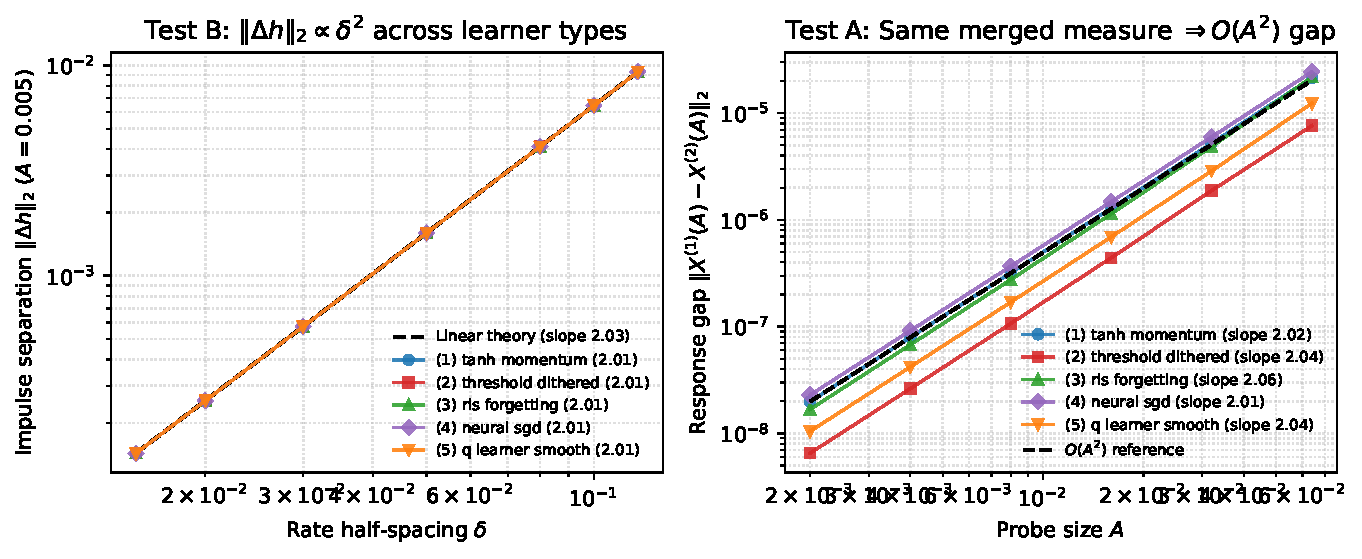
\includegraphics[width=0.92\textwidth]{figs/fig_learners.pdf}
\caption{Left: Test~B, probe-normalised response difference $\|\Delta h\|_2$ against the rate half-spacing $\delta$ at probe size $A=0.005$, five stylized rules and the linear benchmark. Right: Test~A, probe-normalised response gap $\|X^{(1)}(A)-X^{(2)}(A)\|_2/A$ between two economies with the same merged measure against the probe size $A$, with an $O(A)$ reference line (corresponding to an $O(A^2)$ raw gap).}\label{fig:learners}
\end{figure}

Table~\ref{tab:learners} and Figure~\ref{fig:learners} show both where the linear reduction holds and where it breaks down. In Panel~A, for small probes every smooth or dithered rule behaves like the linear model: economies with the same merged measure have raw response gap $O(A^2)$ (slopes $2.011$ to $2.064$) and probe-normalised gap $O(A)$ (slopes $1.011$ to $1.064$), while the response difference and capital lower bound scale as $\delta^2$ (slope $2.007$) and $\delta^{-4}$ (slope $-4.001$), with capital at $\delta=0.05$ within $0.1\%$ of the linear $61.42$. In Panel~B, predictions (a)--(c) pass for all four trained learners: a single exponential explains $R^2\ge0.993$ of each small-probe impulse response, populations with the same merged measure differ by at most $10^{-5}$ in relative response at $A=0.005$, and capital lower bound scales with slopes $-4.014$ to $-3.973$, inside the registered band. The level of capital differs across learners because training sets the response gain.

Panel~C shows where this changes. When the two populations are trained on independent innovation streams, prediction (c) fails: the capital slopes are $-1.75$, $-0.97$, $-1.62$ and $-0.38$. Independently trained populations end with learned gains that differ by sampling error of order $T_{\rm burn}^{-1/2}$, so they differ in merged weight as well as in memory rate, and a difference in weight is cheaper to detect than an $O(\delta^2)$ difference in rates. The $\delta^{-4}$ law therefore prices the separation of memory rates between populations whose feedback weights match; it is not a claim about telling apart any two trained populations. When learning continues during the probe at rate $0.35$, the law survives (slopes $-4.02$ to $-3.98$) and the merged-measure gap rises only to $1.1\times10^{-3}$, so the breakdown we anticipated under prediction (d) did not occur in this design.

The linear theory fails in two further places. First, saturation, adaptive gains and the neural readout leave the small-signal regime once probes exceed $A_{\rm sat}\in[0.751,1.271]$ par units, and the dithered threshold rule leaves it already at $A_{\rm sat}=0.049$, the threshold itself. Second, rules with hard discontinuities are different in kind: an exact dead zone ($\tau=0.05$) or a single-bin lookup does not respond at all to probes smaller than $0.139$ and $0.149$ par units ($\|\Delta h\|_2=0$), concealing those cohorts from small probes altogether. Neither smooth nonlinearity nor hard thresholds offers a cheaper route to separating memory rates than the linear benchmark; populations whose learned weights differ are told apart by their weights, not their rates.

